%% LyX 2.4.2.1 created this file.  For more info, see https://www.lyx.org/.
%% Do not edit unless you really know what you are doing.
\documentclass[12pt,english]{beamer}
\usepackage{mathpazo}
\renewcommand{\familydefault}{\rmdefault}
\usepackage[T1]{fontenc}
\usepackage[latin9]{inputenc}
\setcounter{secnumdepth}{3}
\setcounter{tocdepth}{3}
\usepackage[active]{srcltx}
\usepackage{amsthm}
\usepackage{amsmath} 
\usepackage{amssymb}
\usepackage[authoryear]{natbib}
\usepackage{graphicx}

\makeatletter
%%%%%%%%%%%%%%%%%%%%%%%%%%%%%% Textclass specific LaTeX commands.
% this default might be overridden by plain title style
\newcommand\makebeamertitle{\frame{\maketitle}}%
% (ERT) argument for the TOC
\AtBeginDocument{%
  \let\origtableofcontents=\tableofcontents
  \def\tableofcontents{\@ifnextchar[{\origtableofcontents}{\gobbletableofcontents}}
  \def\gobbletableofcontents#1{\origtableofcontents}
}
\theoremstyle{definition}
\newtheorem*{example*}{\protect\examplename}
\theoremstyle{definition}
\newtheorem*{defn*}{\protect\definitionname}
\theoremstyle{plain}
\newtheorem*{thm*}{\protect\theoremname}

%%%%%%%%%%%%%%%%%%%%%%%%%%%%%% User specified LaTeX commands.
\AtBeginDocument{%
   \let\origtableofcontents=\tableofcontents
   \def\tableofcontents{\@ifnextchar[{\origtableofcontents}{\gobbletableofcontents}}
   \def\gobbletableofcontents#1{\origtableofcontents}
 }\usepackage[english]{babel}
\usepackage{babel}

%\usetheme{Boadilla}
\usetheme{Madrid}
% \usecolortheme{orchid}
\usecolortheme{spruce}
% \usecolortheme{beaver}

\setbeamercovered{transparent}

\usepackage{colortbl}

\usefonttheme[onlymath]{serif}
%%%%%%%%%%%%%%%%%%%%%%%%

% For tables
\usepackage{multirow}
\usepackage{array}
\usepackage{rotating}
\usepackage{longtable}
\usepackage{float}
\usepackage{booktabs}


% For figures
\usepackage{caption}
\usepackage{subcaption}

\makeatother

\usepackage{babel}
\providecommand{\definitionname}{Definition}
\providecommand{\examplename}{Example}
\providecommand{\theoremname}{Theorem}

\begin{document}
\title[Limited]{Models of Limited Dependent Variables}
\author[]{Zhentao Shi}
\date[]{The Chinese University of Hong Kong}

\makebeamertitle



\begin{frame}{Fundamental Task}

        \begin{itemize}
            \item Use $X$ to predict $y$
        \item Beyond continuous random variables
        \begin{itemize}
            \item Binary
            \item Multi-responses 
            \item Integer
            \item Mixed type: censoring, truncation
            \item Self-selection
        \end{itemize}

\bigskip
            
        \item Applied microeconomics
        \item Biostatistics
            
        \end{itemize}
\end{frame}


\section{Binary Choices}
\frame{\sectionpage}




\begin{frame}{Binary Outcome}
    \begin{minipage}{0.6\textwidth} % Left side for text
        \begin{itemize}
            \item Classification
            \item Binary choice:    $y_{i} \in \{ 0, 1\}$
            \begin{itemize}
                \item College entrance
                \item Marriage
                \item Loan decision
            \end{itemize}
        \end{itemize}
    \end{minipage}%
    \hfill
    \begin{minipage}{0.4\textwidth} % Right side for image
        \centering
        
\includegraphics[width=0.8\textwidth]{fig/yin_yang.png}
    \end{minipage}
\end{frame}






\begin{frame}{Linear Probability Models}

\begin{itemize}
    \item Stick to linear regression $y_i = X_i^{'} \beta + \varepsilon_i$
    \item Conditional mean $$\Pr \left[y_{i} = 1 \mid X_{i}\right] = E\left[y_{i} = 1 \mid X_{i}\right] = X_{i}^{'} \beta$$
    \item Error term $\varepsilon _{i} \in \{  - X_{i}^{'} \beta, \, 
    1- X_{i}^{'} \beta \} $ is binary.
    \item Conditional heteroskedastic.
    \item Predicted range: $E\left [y_{i} = 1 \mid X_{i} \right] = X_{i}' \beta$ can go beyond $\left[0,1\right]$.
    \begin{itemize}
        \item $X_{i}^{'} \beta$ is a ``single index''.
    \end{itemize}
\end{itemize}
\end{frame}

\begin{frame}{Generalized Linear Model}
    \begin{itemize}
        \item To ensure predicted probability inside \( [0,1] \), pick some \( G(\cdot ) : \mathbb{R} \to \left[ 0, 1\right] \) to model 
        \[
        E\left( y _{i} = 1 \mid X_{i} \right) = G (X_i^{'} \beta) 
        \]
        \item Popular choices
        \begin{itemize}
           \item Probit: \( G(x) \sim \text{Normal cdf} \)
           \item Logit: \( G\left(x\right) \sim \text{Logistic cdf} \)
        \end{itemize}
        \item Facts about Logistic CDF
        \begin{itemize}
            \item \( \Lambda = \Lambda \left(x\right) = \frac{1}{1 + \exp \left(-x\right)} \)
            \item \( \frac{\mathrm{d} \Lambda }{\mathrm{d} x} = \Lambda \left(1-\Lambda \right) \)
        \end{itemize}
    \end{itemize}
    \begin{picture}(0,0)
        % Adjust the position and scale of the image as needed
        \put(185,-5){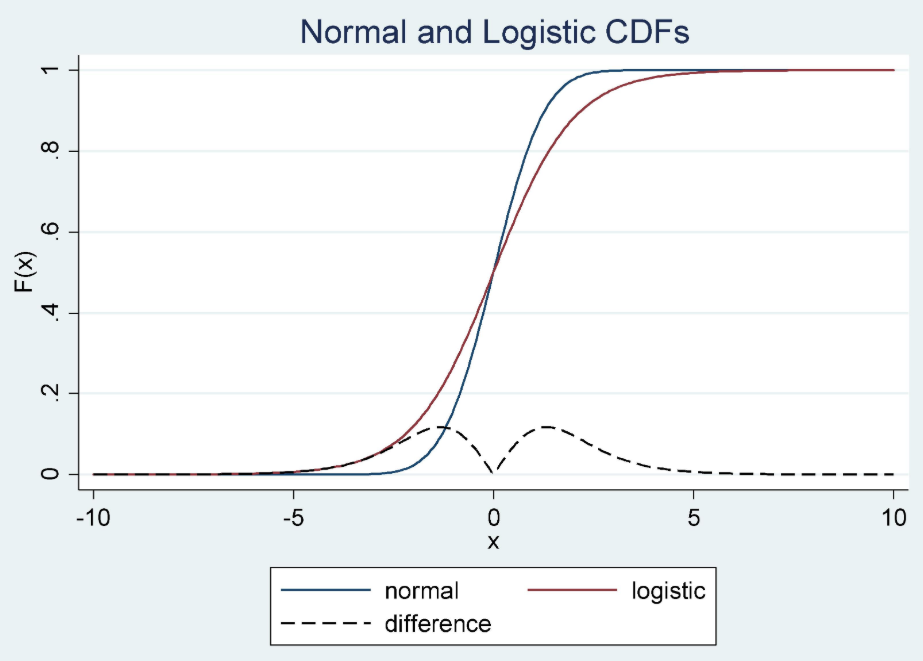
\includegraphics[width=0.45\textwidth]{fig/logistic_normal.png}}
    \end{picture}  
\end{frame}
\begin{frame}{Latent Utility Model}

\begin{itemize}
    \item Latent utility $y^{*} = X_{i}^{'} \beta + \varepsilon _{i}$
    \item Observed outcome $y = \mathbb{I}\left\{ y_{i} ^{*} \ge 0 \right\}$
    \item If $\varepsilon _{i} \mid X_i \sim \text{Logistic}$, then
    \begin{align*}
        \Pr\left(y_i = 1 \mid X_i \right) &= \Pr \left(X_i^{'} \beta + \varepsilon _{i} \ge 0 \mid X_i\right)\\
        & = \Pr \left( - \varepsilon _{i} \le X_{i}^{'} \beta \mid X_{i}\right)\\
        & = \Lambda \left(X_i^{'} \beta\right)
    \end{align*}
\end{itemize}


\end{frame}
\begin{frame}{Log-Likelihood}

A sample of $N$ observations of $(y_i, X_i)$
    \begin{align*}
        L(\beta) &= \prod_{y_i = 1 } \Lambda \left( X_i ^{'} \beta \right)\cdot \prod_{y_i = 0} \left(1 - \Lambda \left(X_{i}^{'} \beta \right)\right)\\
        &= \prod_{i =1}^{N}\left\{ \Lambda \left(X_i^{'} \beta \right) \right\} ^{y_i} \left\{ 1- \Lambda \left( X_{i}^{'} \beta \right) \right\} ^{1-y_{i}}
    \end{align*}

Log-likelihood
    \[\log L\left( \beta \right) = \sum_{i =1}^{N} \left\{ y_i \log \left( \Lambda \left( X_{i}^{'}\beta \right) \right) + \left( 1 - y_{n} \right)  \log \left( 1 - \Lambda \left( X_i \beta \right) \right)\right\}\]
    
    
\end{frame}

\begin{frame}{Properties}


    \begin{itemize}
    \item The score
    \begin{align*}
        S_N(\beta) &= \sum_{i = 1}^{N}\left\{ \frac{y_i}{\Lambda_i}\cdot \Lambda_{i}\left( 1 - \Lambda _i \right) X_{i} - \frac{\left( 1- y_{i} \right)}{1 - \Lambda_{i}} \cdot \Lambda_{i} \left( 1-\Lambda_{i} \right) X_{i}\right\}\\
        &= \sum_{i=1}^{N}\left\{ y_{i} \left( 1- \Lambda_{i} \right) - \left( 1-y_{i} \right) \Lambda_{i}\right\} X_{i}\\
        &= \sum_{i =1}^{N}\left( y_{i} - \Lambda _{i} \right)X_{i} 
    \end{align*}
    \item Negative-definite second derivative
    \[\frac{\partial L \left( \beta \right)}{\partial \beta \partial \beta ^{'}} = - \sum_{i=1}^{N} \Lambda_{i}\left( 1 - \Lambda_{i} \right) X_{i} X_{i}'.\]

        \item Globally concavity implies uniqueness of maximizer.
    \end{itemize}
\end{frame}


\begin{frame}{Goodness of Fit for Binary Classification}
     $$\text{McFadden} R^{2} = 1- \log L_{1} / \log L_{0}$$
    \begin{itemize}
        \item $\log L_{1}$: maximum of likelihood
        \item $\log L_{0}$: the null model (no $X$, intercept only)
            \[\log L_{0} = N_1 \log \hat{p}_1 + \left( N-N_{1} \right)\log \left( 1- \hat{p}_1 \right) \]
            where $\hat{p}_1 = N_{1} / N$
        \item $\log L_{0} < \log L_{1} < 0 \Rightarrow \frac{\log L_{1}}{\log L_{0}} \in \left[0,1  \right]$                
    \end{itemize}
\end{frame}
\begin{frame}{Prediction and Evaluation}
   Natural prediction: \[\hat{y_{i}} = 1 \,\text{if}\, \Pr\left( y_{i} \mid X_{i} \right) \ge 0.5\]

   Outcomes: $n_{11}$: correct positive; $n_{01}$: false positive
    \begin{table}
        \centering
        \begin{tabular}{rr|ccc}
            & & $\hat{y}_i = 0$ & $1$ & Total \\
            \hline
              & $y_{i}=0$ & $n_{00}$ & $n_{01}$ & $N_{0}$ \\
            & $1$ & $n_{10}$ & $n_{11}$ & $N_{1}$ \\
            \hline
            & Total &&& $N$ 
        \end{tabular}
    \end{table}
    \begin{itemize}
        \item Hendrick-Merton: $\frac{n_{00}}{N_{0}} + \frac{n_{11}}{N_{1}}$
        \item Kuiper Score: $\frac{n_{11}}{N_{1}} - \frac{n_{01}}{N_{0}}$
    \end{itemize}
\end{frame}




\section{Multiple Choices}
\frame{\sectionpage}


\begin{frame}{Ordered Response}
    \begin{itemize}
        \item More than two categories
        \item Categories are naturally ordered
        \begin{itemize}
            \item e.g.~Top 2, C9, 985, 211, others
        \end{itemize}
        \item Latent utility: $$y_{i}^{*} = X_{i}' \beta + \varepsilon_{i}$$ while the observed outcome  $$y_{i} = j, \, \text{if}\, r_{j} < y_{i}^{*} \le r_{j+1}$$
        
    \end{itemize}
\end{frame}

\begin{frame}{Thresholds}
    \begin{itemize}
        \item Normalization is needed for identification
        \item $M$ categories
        \item $\gamma_{1} = - \infty,\, \gamma_{M+1} = + \infty, \, \gamma_{2} = 0$
        \bigskip
        \item Unknown parameters: $\left( \beta, \gamma_{3}, \dots, \gamma_{M} \right)$
    \end{itemize}
    \begin{align*}
        P_{ij} & = \Pr\left( \gamma_{j} < y_{i}^{*} \le \gamma_{j+1} \mid X_{i}\right)\\
        & = \Pr \left( y_{i}^{*} \le \gamma_{j+1} \mid X_{i} \right) - \Pr \left( \gamma_{j} \le y_{i}^{*} \mid X_{i} \right)\\
        & = \Pr \left( \varepsilon_{i} \le \gamma_{j+1} - X_{i}^{'} \beta \right) - \Pr \left( - \varepsilon_{i} \le X_{i}^{'} \beta - \gamma_{j} \mid X_{i} \right)
    \end{align*}
\end{frame}

\begin{frame}{Likelihood}
    \begin{itemize}
        \item $\varepsilon_{i} \mid X_{i}$ can be either logistic or normal
    \end{itemize}
    \[ \Pr \left( y_i = j \right) = \sum_{j=1}^{M} P_{ij} \mathbb{I}\left\{ y_j = j \right\}\]
    \[ L\left( \theta \right) = \prod_{i =1} ^{N} \Pr \left( y_j = j \right)\]
\end{frame}

\begin{frame}{Multinomial Choice}
    \begin{itemize}
        \item Hong Kong to Guangzhou\\
        bus, train, or plane?
        \item Choice specific regressors $X_{ij}$
        \begin{itemize}
            \item distance to stations
        \end{itemize}
        \item Choice in variant regressors $x_{i}$
        \begin{itemize}
            \item motion sickness
        \end{itemize}
        \item individual-choice utility\\
        $u_{ij} = X_{ij}^{'} \beta + x_{i}^{'} \beta_{j}$
    \end{itemize}    
\end{frame}

\begin{frame}{Latent Utility}
    \begin{itemize}
        \item $y_{ij}^{*} = \mu_{ij} + \varepsilon _{ij}$, for $\left(\varepsilon_{ij}\right)_{j=1}^{M}$
        \item $y_{j} = \mathbb{I}\left\{ j: y_{ij}^{*} \ge y_{ik},\,\text{for}\, k = 1, \dots, M \right\}$
        \item $\Pr \left( y_{j} = j \mid X_{i} \right) = \Pr \left( y_{ij}^{*} \ge y_{i1}^{*}, \dots, y_{ij}^{*} \ge y_{iM}^{*} \right)$\\
        depends on the joint distribution of $\left( \varepsilon_{ij} \right)_{j=1}^{M}$
        \item if $\varepsilon _{ij} \sim $Type $\text{I}$ extreme value distribution and $\varepsilon_{ij}$ i.i.d. across choices, then
        \[\Pr\left( y_{ij} = j \mid \mu_{i1}, \dots, \mu_{iM} \right)= \frac{\exp\left( \mu_{ij}\right)}{\sum_{k=1}^{M}\exp \left( \mu_{ik}\right)}\]
    \end{itemize}
\end{frame}
\begin{frame}{Normalization}
    \begin{itemize}
        \item $\mu_{i1} = 0$ for all $i$
        \item Equivalent to $\beta_{1} = 0$ (including intercept)
        \item parameters: $\left( \beta_1, \beta_2, \beta_3, \dots, \beta_M\right)$
    \end{itemize}
    \[L\left( \theta \right) = \prod_{i=1}^{n} \left\{ \sum_{j=1}^{M} \mathbb{I} \left( y_{ij} = j \right)\left( \frac{\exp \left( \mu_{ij} \right)}{H \sum_{k=2}^{M} \exp \left( \mu_{ik} \right)} \right) \right\}\]
\end{frame}

\begin{frame}{Independence of Irrelevant Alternative}
    \begin{itemize}
        \item Assume $\varepsilon_{ij}$ i.i.d. across choices
        \item Red bus and blue bus have no essential difference
        \item Must pay attention to the specification of choice set
    \end{itemize}
\end{frame}
\begin{frame}{Poisson MLE}
\begin{itemize}
    \item Log-likelihood function of an $N$-observation sample:
    \[
    \ell_N(\beta) = \log \Pr( \mathbf{y} | \mathbf{X}; \beta ) = -\sum_{i=1}^n \exp(X_i'\beta) + \sum_{i=1}^n y_i X_i'\beta.
    \]
    
    \item Score:
    \[
    s_N(\beta) = \frac{\partial \ell(\beta)}{\partial \beta} = -\sum_{i=1}^n \exp(X_i'\beta)X_i + \sum_{i=1}^n y_i x_i.
    \]

    \item Second derivative is negative definite:
    \[
    \frac{\partial^2 \ell(\beta)}{\partial \beta \partial \beta'} = -\sum_{i=1}^n \exp(X_i'\beta) X_i X_i'
    \]

    \item \( \ell_N(\beta) \) is strictly concave in \( \beta \).

\end{itemize}
\end{frame}


\section{Integer Outcomes}
\frame{\sectionpage}


\begin{frame}{Counting Model}
\begin{itemize}
    \item Outcomes take non-negative integers
    \begin{itemize}
        \item Number of children
        \item Number of hospital visits
        \item Number of patents
    \end{itemize}
    \item Poisson model: 
$y \sim \text{Poisson}(\lambda)$:
$$
\Pr(y = k) = \frac{\mathrm{e}^{-\lambda} \lambda^k}{k!}, \mathrm{ for }\, \, k=0,1,2,\ldots
$$
    \item Poisson regression: single index $\lambda_i = X_i'\beta$ gives log-likelihood
$$
\log \Pr(y_i | X_i) =  -\exp(X_i'\beta) + y_i\cdot X_i'\beta - \log k!
$$
\end{itemize}
\end{frame}



\begin{frame}{Pseudo Poisson MLE}

\begin{itemize}
    \item Conditional mean model $E[y|X] = \exp (X'\beta)$
    \item If $y$ is continuously distributed, the Poisson model must be misspecified
    \item e.g., Bilateral international trade between pairs of countries.
\end{itemize}
\end{frame}


\end{document}